\maketitle

\begin{frame}
  \frametitle{new CMS coordinator}
  Welcome to Loukas Gouskos as new IML coordinator for CMS

  {~}

  {~}

  \begin{columns}
    \begin{column}{.4\textwidth}
      
\includegraphics[width=\textwidth]{./loukas.png}
    \end{column}
  \end{columns}
\end{frame}

\begin{frame}
  \frametitle{IML workshops}
  Following the annual workshop, we're digesting the feedback forms for the planning of next year's workshop. Overall positive feedback.

  \begin{block}{IML workshop 2020}
    Next year's workshop possibly early June to avoid collision with ``Connecting the Dots'' and ``Dark Machines''.

    More news once things are fixed.
  \end{block}
\end{frame}

\begin{frame}[t]
  \frametitle{Participation}
  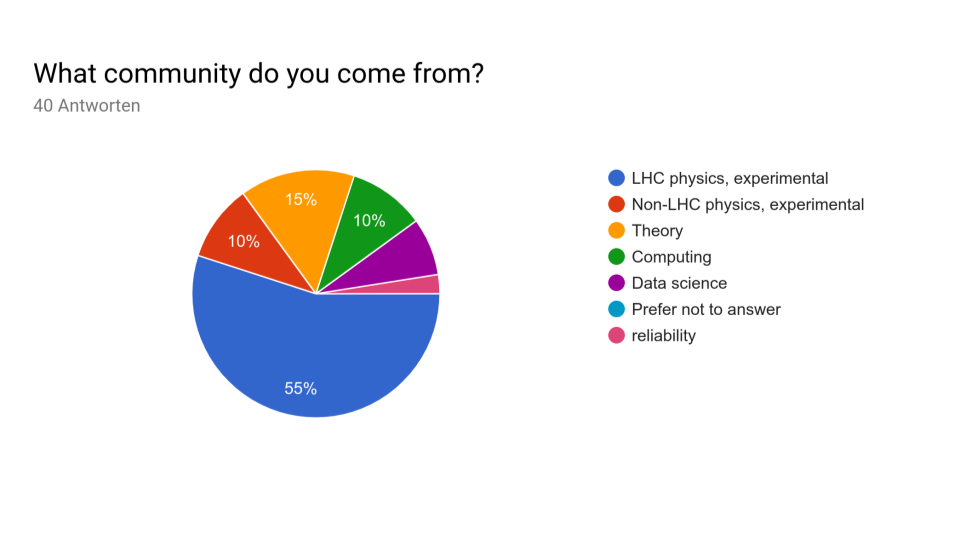
\includegraphics[width=.62\textwidth]{community.png}
  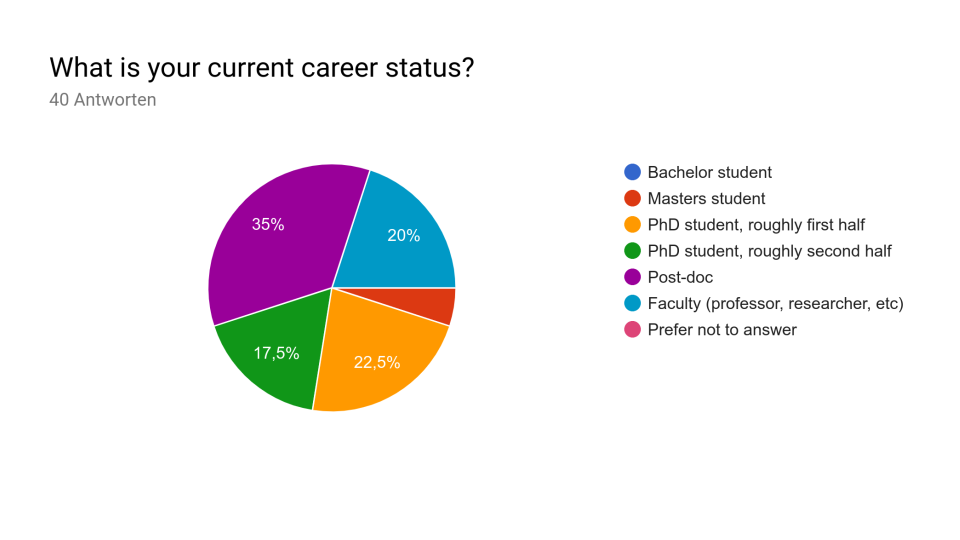
\includegraphics[width=.62\textwidth]{community2.png}
  % 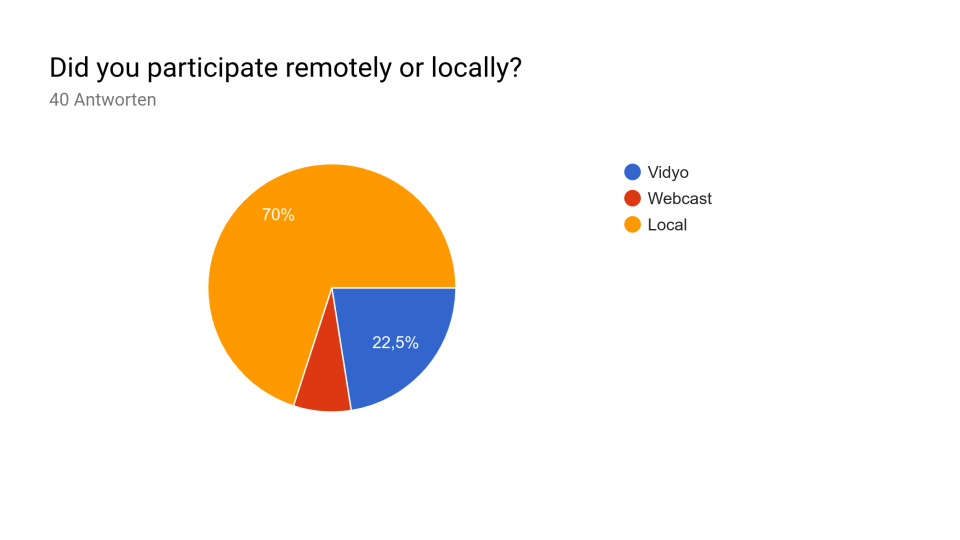
\includegraphics[width=.62\textwidth]{local_remote.png}
  \only<2>{
    \vspace{-.6\textheight}
    \begin{columns}
      \begin{column}{.7\textwidth}
        \begin{alertblock}{ }
          about half of the participants not LHC physicists
        \end{alertblock}
      \end{column}
    \end{columns}
  }
\end{frame}
\begin{frame}[t]
  \frametitle{Participation}
  % 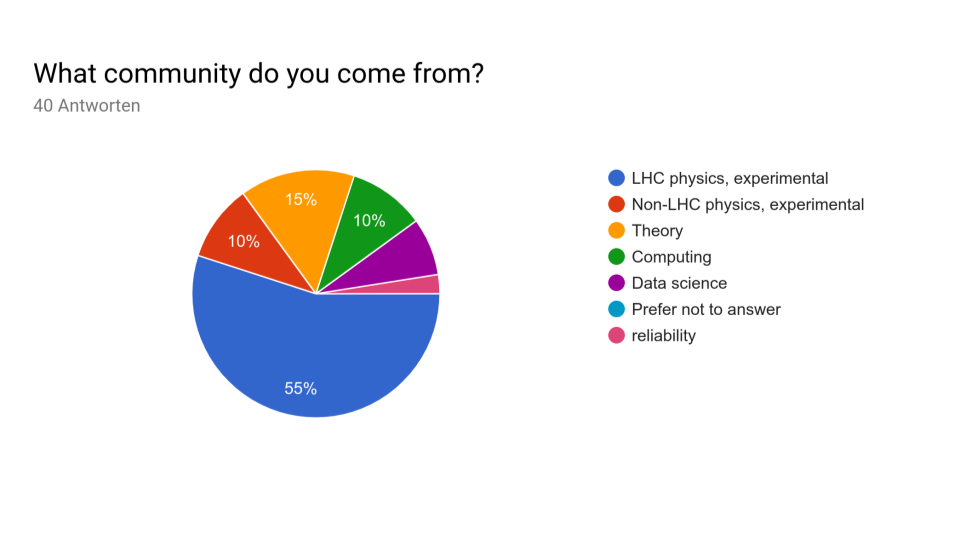
\includegraphics[width=.62\textwidth]{community.png}
  % 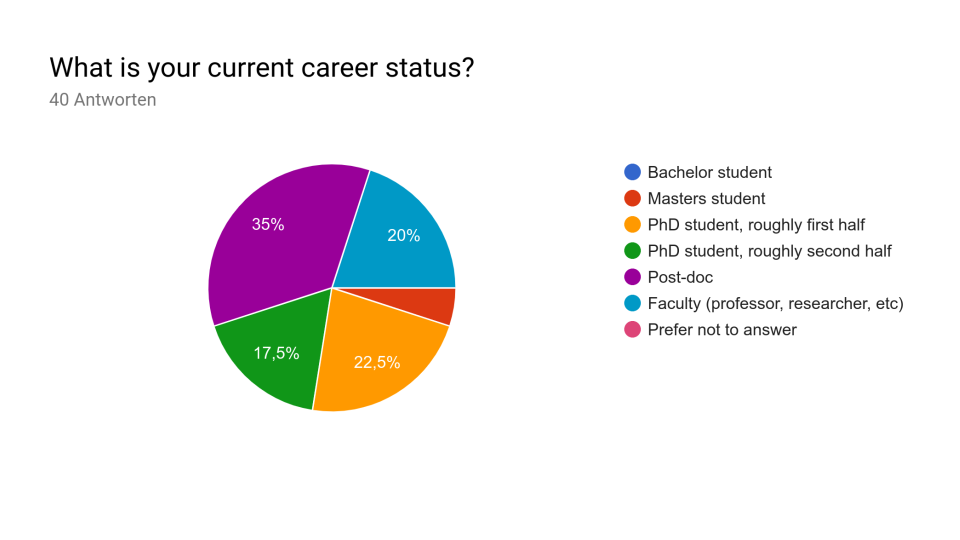
\includegraphics[width=.62\textwidth]{community2.png}
  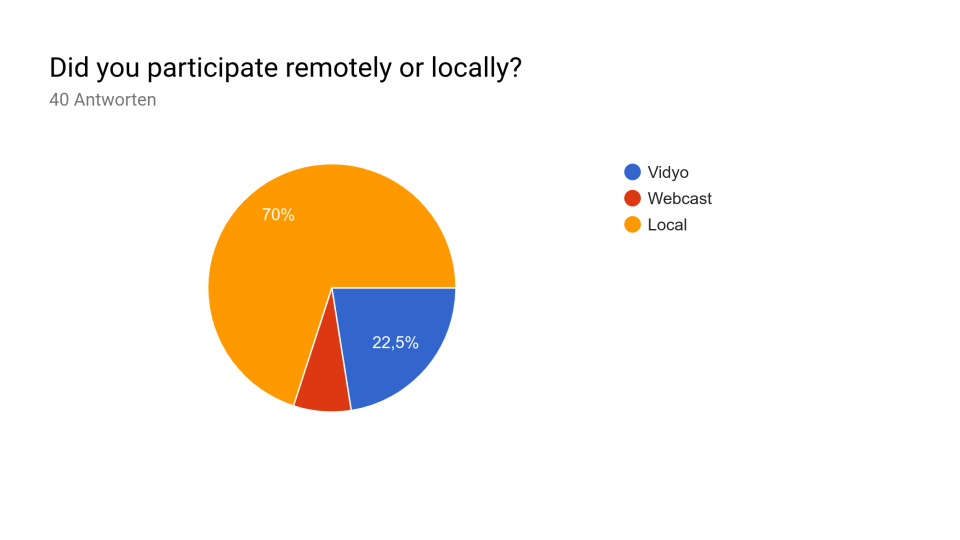
\includegraphics[width=.62\textwidth]{local_remote.png}
  \only<2>{
    \vspace{-.1\textheight}
    \begin{columns}
      \begin{column}{.7\textwidth}
        \begin{alertblock}{ }
          possibility for remote participation is used
        \end{alertblock}
      \end{column}
    \end{columns}
  }
\end{frame}
\begin{frame}[t]
  \frametitle{Industry session}
  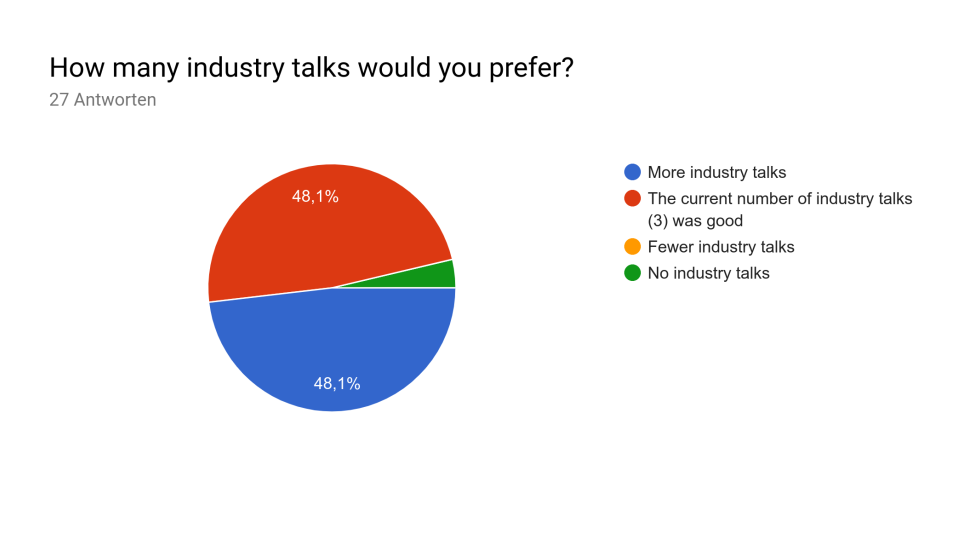
\includegraphics[width=.62\textwidth]{industry.png}
  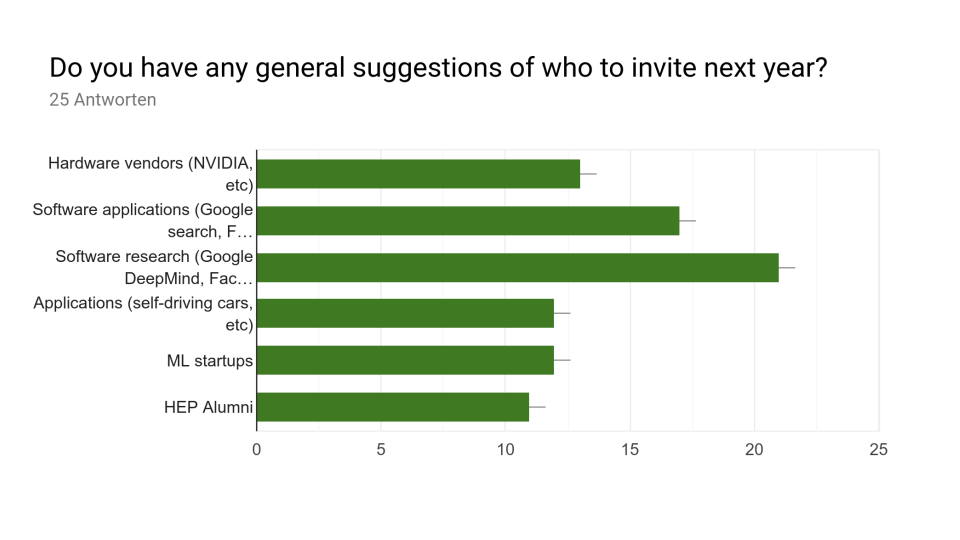
\includegraphics[width=.62\textwidth]{industry2.png}
  \only<2>{
    \vspace{-.6\textheight}
    \begin{columns}
      \begin{column}{.7\textwidth}
        \begin{alertblock}{ }
          Will look for 3 to 4 industry talks from mixed companies
        \end{alertblock}
      \end{column}
    \end{columns}
  }
\end{frame}
\begin{frame}[t]
  \frametitle{Invited talks}
  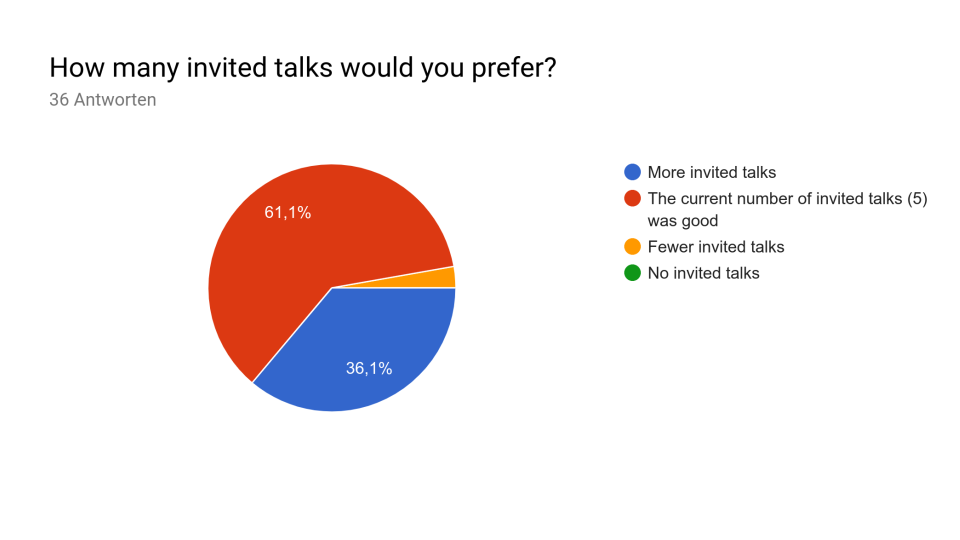
\includegraphics[width=.62\textwidth]{invited.png}
  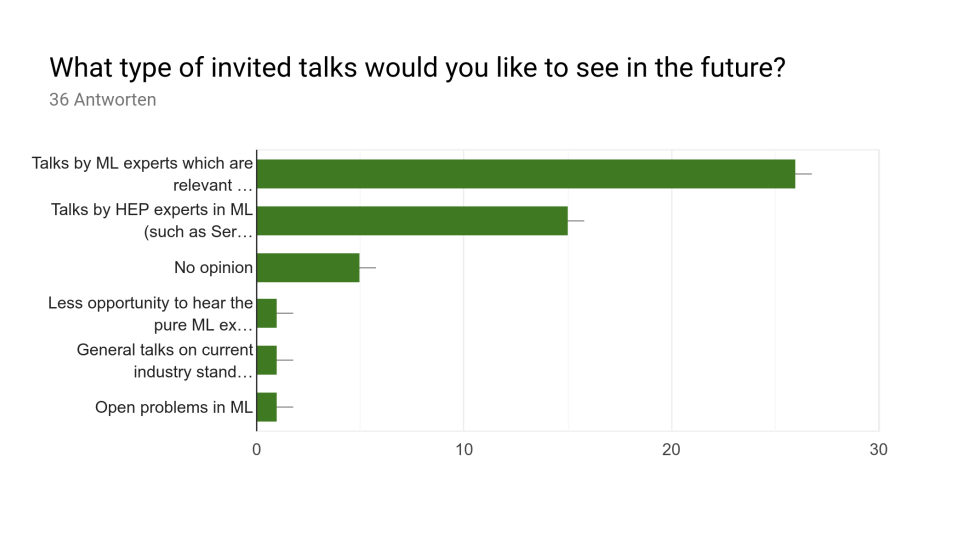
\includegraphics[width=.62\textwidth]{invited2.png}
  \only<2>{
    \vspace{-.6\textheight}
    \begin{columns}
      \begin{column}{.7\textwidth}
        \begin{alertblock}{  }
          Some preference for ML experts over HEP experts $\to$ keep inviting both
        \end{alertblock}
      \end{column}
    \end{columns}
  }
\end{frame}
\begin{frame}[t]
  \frametitle{Physics sessions}
  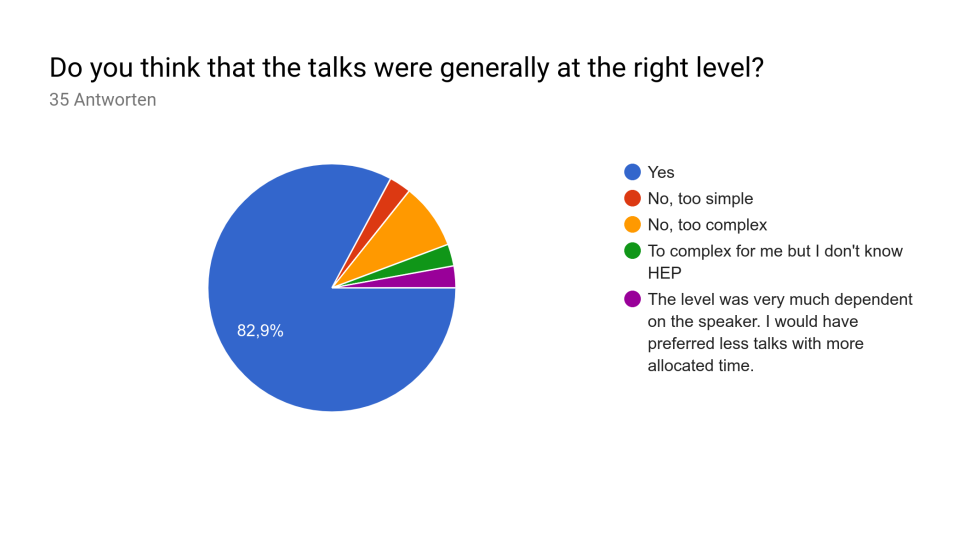
\includegraphics[width=.62\textwidth]{physics.png}
  \only<2>{
    \vspace{-.1\textheight}
    \begin{columns}
      \begin{column}{.7\textwidth}
        \begin{alertblock}{ }
          Obviously varies from talk to talk, but overall you managed to prepare your presentations on the right level.

          Thanks you!
        \end{alertblock}
      \end{column}
    \end{columns}
  }
\end{frame}
\begin{frame}[t]
  \frametitle{Tutorials}
  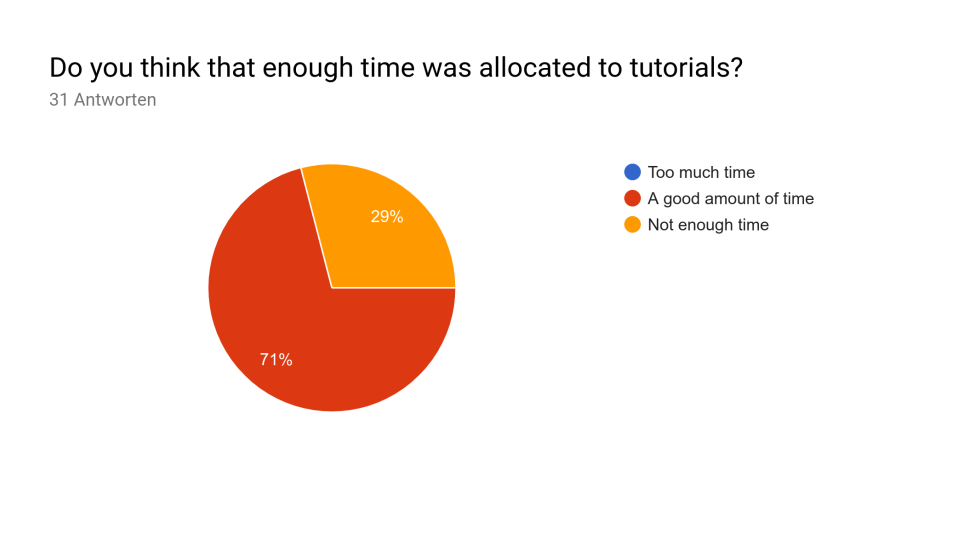
\includegraphics[width=.62\textwidth]{tutorials.png}
\end{frame}
\begin{frame}[t]
  \frametitle{Tutorials}
  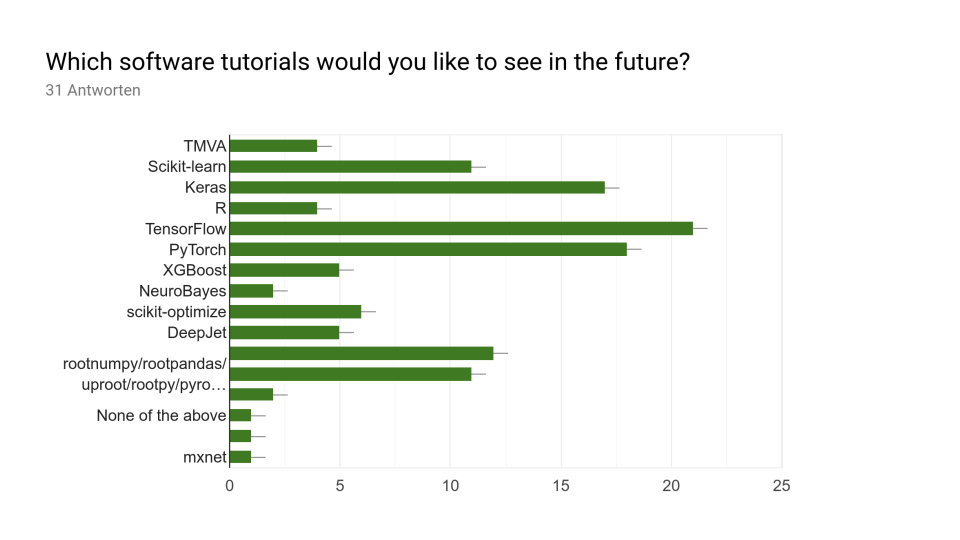
\includegraphics[width=.62\textwidth]{tutorials2.png}
  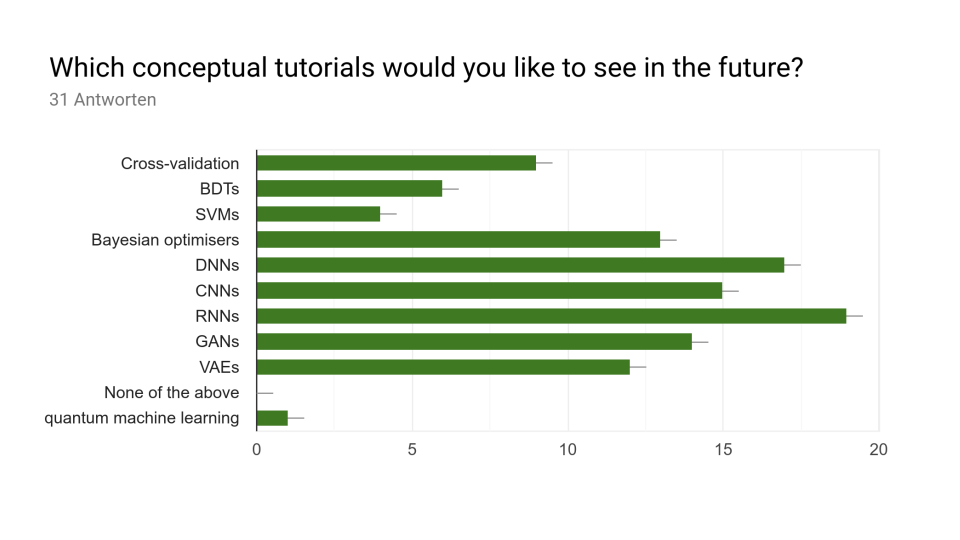
\includegraphics[width=.62\textwidth]{tutorials3.png}
  \only<2>{
    \vspace{-.6\textheight}
    \begin{columns}
      \begin{column}{.7\textwidth}
        \begin{alertblock}{ }
          Hard to get the time slots for tutorials right (not everybody will attend). Some suggestions to have the tutorials before rather than after the other workshop parts.
        \end{alertblock}
      \end{column}
    \end{columns}
  }
\end{frame}

\begin{frame}
  \frametitle{Bonus items on the agenda}
  \begin{columns}
    \begin{column}{.48\textwidth}
      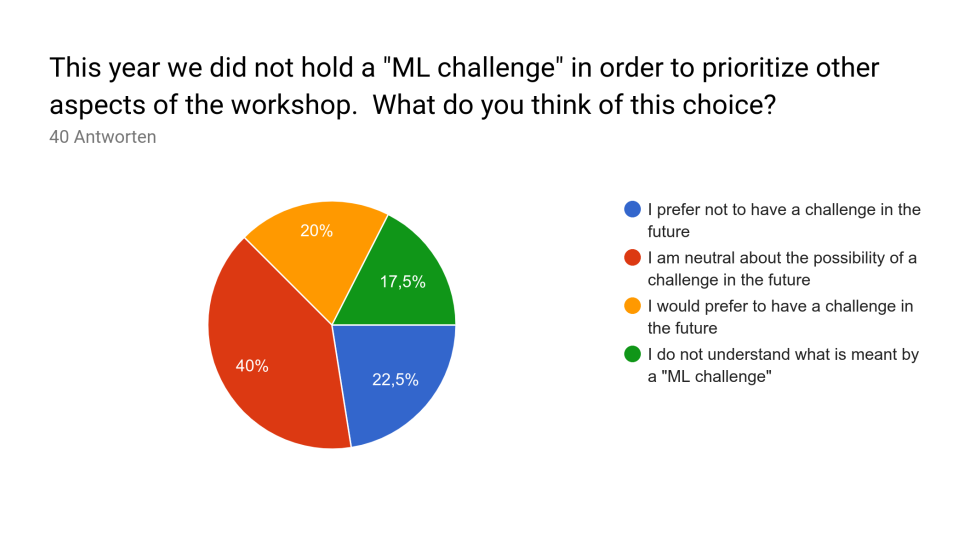
\includegraphics[width=\textwidth]{./challenge.png}

      {\footnotesize{

        Challenge: a data mining task is published, participants should solve it with ML, maximising a figure of merit. Like Kaggle.

      }}
    \end{column}
    \begin{column}{.48\textwidth}
      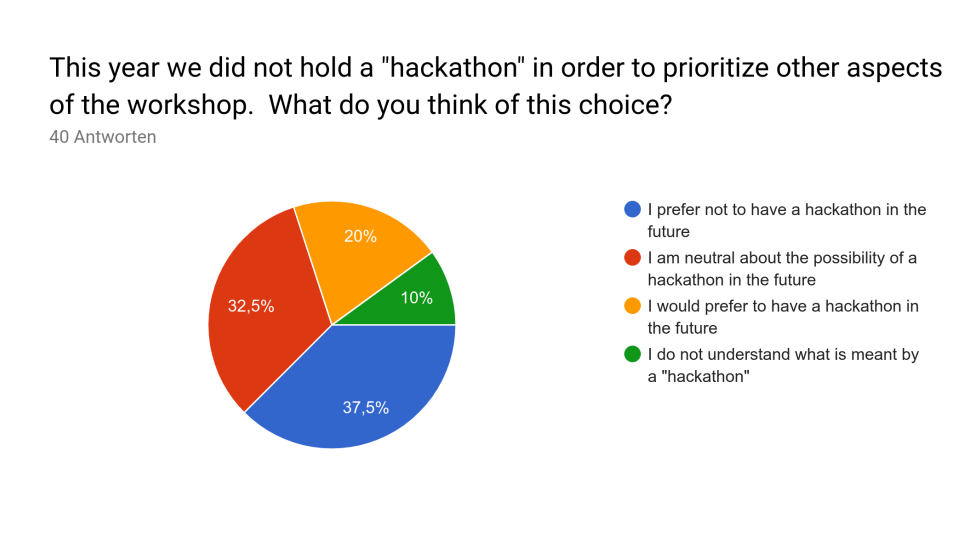
\includegraphics[width=\textwidth]{./hackathon.png}

      {\footnotesize{

        Hackathon: participants sit in a room, no talks / discussion, just collaborating in working on some task. Ability to ask others for help, suggestions.

      }}
    \end{column}
  \end{columns}

\end{frame}

\begin{frame}
  \frametitle{time budget}
  \begin{itemize}
    \item In most categories the feedback asks for the same amount of time or some more
    \item At the same time, the feedback says the the overall workshop length is about right
    \newline (didn't look into the correlation of these questions yet)
  \end{itemize}
\end{frame}

\begin{frame}
  \begin{columns}
    \begin{column}{.98\textwidth}
      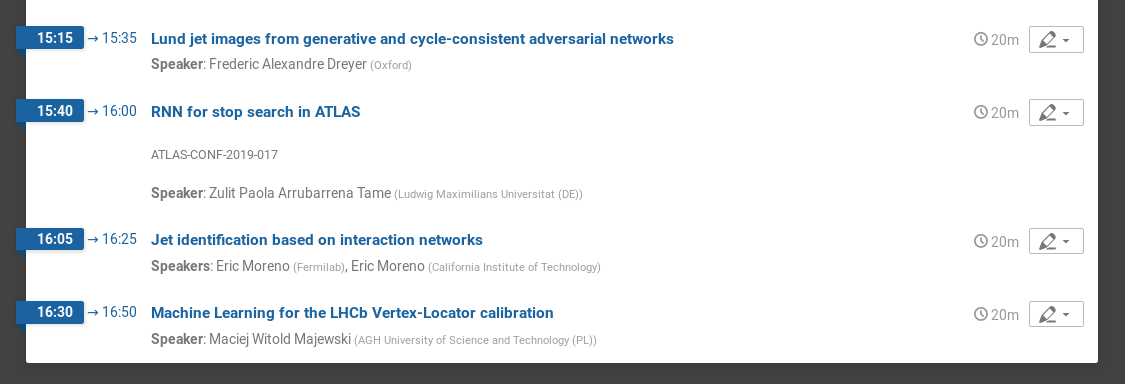
\includegraphics[width=\textwidth]{./agenda.png}
    \end{column}
  \end{columns}
\end{frame}

\appendix
\begin{frame}

  \vspace{.3\textheight}

  \IfFileExists{./QR2.png}{
    \footnotesize{slides (excl.\ cern logo) will appear on}

    \gitlablink
\includegraphics[width=.2\textwidth]{./QR2.png}
  }{}
\end{frame}
